\section{Results and discussion} \label{Results-and-discussion}
The molar fraction of the heavy metal (HM) 
in the initial fuel was kept constant and equal to 12.5 mole\% for all cases (see Table~\ref{tab:table4}). 
Additionally, the initial fissile material fraction was increased for the five fuel 
salt compositions until the \gls{SD-TMSR} reactor was sufficiently critical at 
the Beginning Of Life (BOL).
\subsection{Thorium feed mechanism}
The thorium feed mechanism continuously feeds thorium from the external stockpile and 
$^{233}$U from the \texttt{Pa-decay tank}.
Figure~\ref{fig:keff1} illustrates the effective multiplication factor 
dynamics during reactor operation for the thorium feed mechanism. As shown in 
Figure~\ref{fig:keff1}, the effective multiplication factor ($k_{eff}$) 
decreases sharply during the first 25 \gls{EFPY} of reactor operation for the first 
four cases. $k_{eff}$ decreases as a result of depletion of the initial 
fissile materials and production of poisonous fission products (FPs). The amount of $^{233}$U generated in 
the SD-TMSR is not enough to maintain the reactor criticality and 
counteract parasitic neutron absorption. Thus, the 
reactor becomes subcritical relatively quickly for alternative startup 
compositions, for example, $\approx$ $4$ years in the \gls{TRU} case and $\approx$ $12$ 
years in the reactor-grade Pu case. For U-233 case, 
the continuous feed flow of thorium and $^{233}$U from the \texttt{Pa-decay tank} helps to operate the 
\gls{SD-TMSR} for a full lifetime (60 year) (Figure~\ref{fig:keff1} (U-233 case)).
Notably, the molar fractions of \gls{HALEU} and reactor-grade Pu in the initial fuel composition were increased
more. Consequently, the initial $k_{eff}$ for these cases increased (Figure~\ref{fig:keff1} (HALEU and reactor-grade Pu cases)).
For the HALEU fuel salt, the amount of $^{233}$U generated in the SD-TMSR after a few years is insufficient to counteract the absorption of the (non-fissile) $^{238}$U added at start-up after much of the original $^{235}$U is depleted. Consequently, the core becomes subcritical after $\approx$ $6$ years of operation.
For the reactor-grade Pu fuel salt, the core becomes subcritical after $\approx$ $12$ years because the amount of $^{233}$U generated is not sufficient to counteract the neutron absorption in the non-fissile plutonium isotopes after much of the $^{239}$Pu and $^{241}$Pu is depleted \cite{betzler2016modeling}.

\begin{figure}
	\centering
	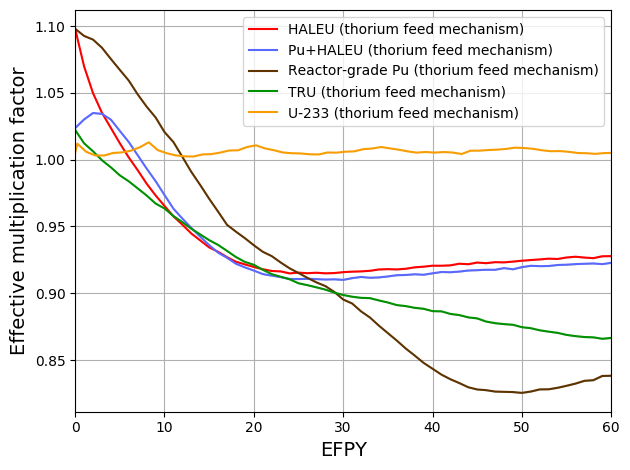
\includegraphics[width=\textwidth]{keff1.png}
		\vspace{-0.5in}
	\caption{The change of the effective multiplication factor during 60 \gls{EFPY} of reactor operation for thorium feed mechanism (confidence interval $\pm\sigma$ is shaded).} 
	\label{fig:keff1}
\end{figure}

\subsection{Non-thorium feed mechanism}
The non-thorium feed mechanism continuously feeds 
$^{233}$U from the \texttt{Pa-decay tank} and external heavy metals (\gls{HALEU}, Pu mixed with \gls{HALEU}, reactor-grade Pu, \gls{TRU}).
Under the non-thorium feed mechanism, four different initial fissile materials are studied: \gls{HALEU}, Pu mixed with \gls{HALEU}, reactor-grade Pu, and \gls{TRU}. The continuous feed of $^{233}$U 
without $^{232}$Th will lead to a supercritical reactor, thus the $^{233}$U case 
is excluded from the non-thorium feed mechanism study.
Figure~\ref{fig:keff2} shows the change of the effective multiplication factor 
during 60 \gls{EFPY} of reactor operation for the non-thorium feed mechanism. Both the reactor-grade Pu and TRU cases 
show promising results relative to the other two cases (HALEU and Pu+HALEU) (see Figure~\ref{fig:keff2}). 
\begin{figure}
	\centering
	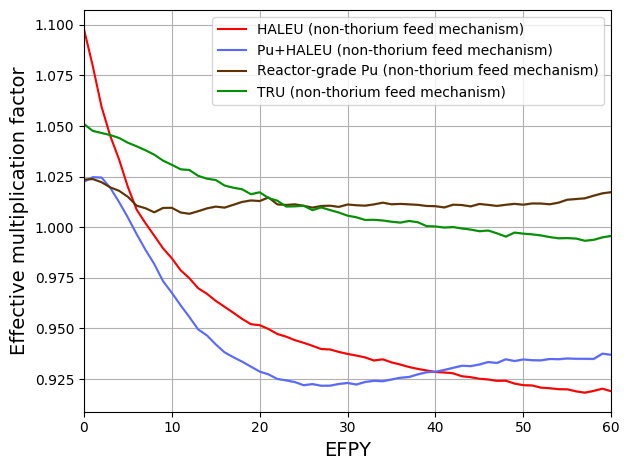
\includegraphics[width=\textwidth]{keff2.png}
			\vspace{-0.5in}
	\caption{The change of the effective multiplication factor during 60 
	\gls{EFPY} of reactor operation for non-thorium feed mechanism (confidence 
	interval $\pm\sigma$ is shaded).} 
	\label{fig:keff2}
\end{figure}
For the reactor-grade Pu case, the amount of $^{233}$U generated in the \gls{SD-TMSR}, in addition to the external feed flow of Pu, is sufficient to maintain the reactor criticality and counteract the neutron absorption in the initial non-fissile isotopes and FPs. 
For the \gls{TRU} fuel salt, the amount of 
$^{233}$U and the external feed flow of TRU is barely enough to operate the 
reactor for a long period of time ($\approx$ $40$ years) without any 
external feed of $^{233}$U ($^{233}$U used only from the \texttt{Pa-decay tank}). Nevertheless, $k_{eff}$ decreases with the burnup 
because of the \glspl{MA}\footnote{In the present work, the minor actinides 
(MA) include Np, Am, and Cm.} accumulating in the core as a result of 
continuous TRU feed. As shown in Figure~\ref{fig:keff2}, the HALEU and Pu+HALEU 
fuel are less attractive for the non-thorium feed mechanism. The continuous HALEU 
feed increases the amount of fertile $^{238}$U and consequently, reduces the 
feasibility of such fissile materials. According to the $k_{eff}$ 
results, reactor-grade Pu and TRU are the only alternative fissile materials that  
can be used to startup and maintain operation of the \gls{SD-TMSR}.

\subsection{Reactor-grade Pu, TRU, and $^{233}$U initial fuel}
In this section, the simulation of the SD-TMSR with reactor-grade Pu and TRU 
fissile materials is discussed. Additionally, the previously studied $^{233}$U 
case is listed for comparison \cite{ashraf2019whole_core}. 
Figure~\ref{fig:refillCCC} demonstrates the dynamics of the heavy metal refill 
rate during 60 \gls{EFPY} of the SD-TMSR operation. The heavy metal refill 
rate was adjusted to maintain criticality and the total fuel mass 
almost constant\footnote{The variation of the total fuel mass is less than 
$0.1\%$} during reactor operation. In the $^{233}$U case, the mean values of 
$^{233}$U and $^{232}$Th refill rate are $1.77$ and $2.21$ $kg/d$, 
respectively. Similarly, in the reactor-grade Pu case, the mean values of 
$^{233}$U and Pu refill rate are $0.75$ and $2.75$ $kg/d$, respectively. For  
the TRU case, the mean values of $^{233}$U and TRU refill rate are $0.90$ and 
$2.0$ $kg/d$, respectively.
\begin{figure}
	\centering
	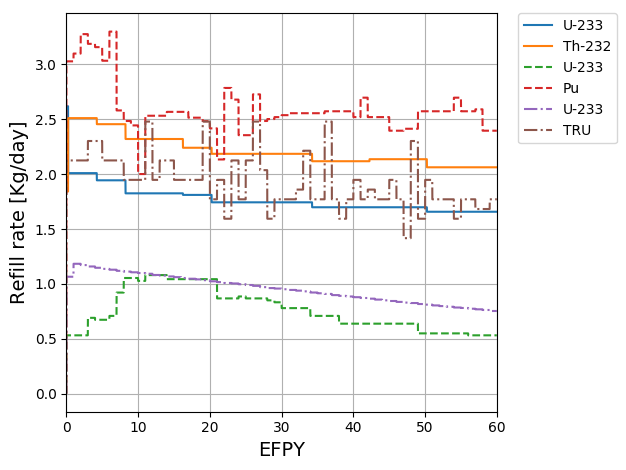
\includegraphics[width=\textwidth]{refillCCC.png}
			\vspace{-0.5in}
	\caption{Dynamics of heavy metal refill rate during 60 \gls{EFPY} of 
		reactor operation. Solid lines for the $^{233}$U case, dashed lines for the
		reactor-grade Pu case, and dotted lines for the TRU case.}
	\label{fig:refillCCC}
\end{figure}

Figures~\ref{fig:inventoryCCCC} and~\ref{fig:inventoryPu_TRUCCC} demonstrate 
the evolution of important nuclide inventories for the $^{233}$U, Pu, and TRU cases 
respectively. For the $^{233}$U case (Figure~\ref{fig:inventoryCCCC}), the mass of Pa in the fuel salt is almost constant and reaches 
$17.8$  $kg$ at the end of the operation time. 
Additionally, the mass of minor actinides (MA) and Pu increases with time. The level of Pu in the fuel salt correlates with the mass of the MA; however, MA need more time to reach equilibrium than Pu. Uranium inventory increases during 
operation and reaches equilibrium after $\approx$ $27$ years. Figure~\ref{fig:inventoryCCCC} shows that refueling the core with thorium helps 
maintain an almost constant inventory throughout the full operation time. 
For the Pu and TRU cases (Figure~\ref{fig:inventoryPu_TRUCCC}), the Pa extraction time was selected to be 30 s 
to avoid poisoning the core. Figure~\ref{fig:inventoryPu_TRUCCC} shows that the mass of Pa in the fuel salt 
is relatively low when compared to Pa mass in the $^{233}$U case (Figure~\ref{fig:inventoryCCCC}). Major 
elements for all three cases reach the equilibrium state after $\approx$ $30$ 
years (see Figure~\ref{fig:inventoryCCCC} and~\ref{fig:inventoryPu_TRUCCC}).
\begin{figure}
	\centering
	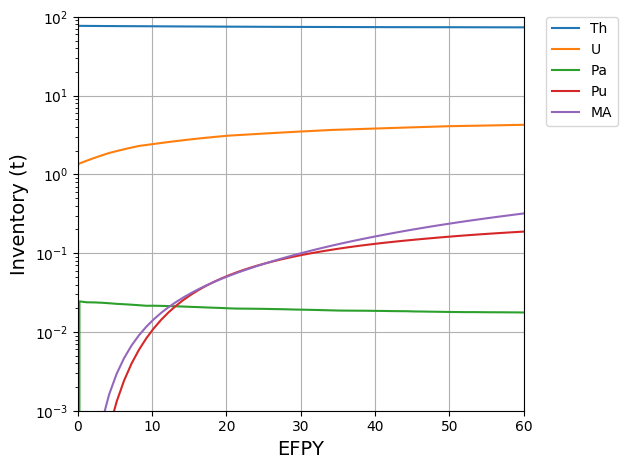
\includegraphics[width=\textwidth]{inventoryCCCC.png}
	\vspace{-0.4in}
	\caption{Evolution of important nuclide inventories for $^{233}$U 
		startup fuel (MA involves Np, Am, Cm) \cite{ashraf2019whole_core}.}
	\label{fig:inventoryCCCC}
\end{figure}
\begin{figure}
	\centering
	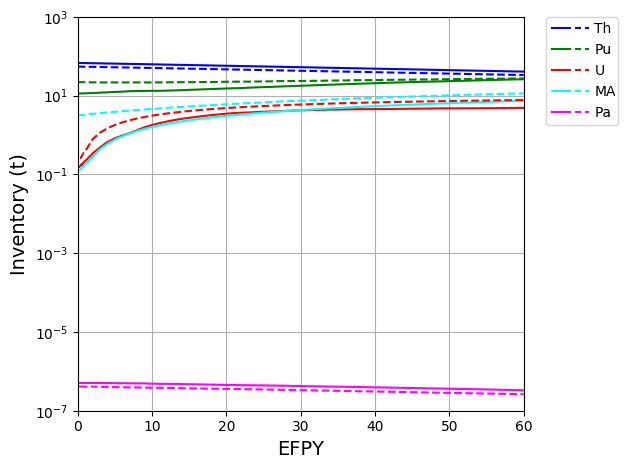
\includegraphics[width=\textwidth]{inventoryPu_TRUCCC.png}
	\vspace{-0.5in}
	\caption{Evolution of important nuclide inventories for the 
		reactor-grade Pu case (solid lines) and for the TRU case (dashed lines).}
	\label{fig:inventoryPu_TRUCCC}
\end{figure}

Figure~\ref{fig:Th232CC} illustrates the variation of thorium inventory in the 
fuel salt for the $^{233}$U, reactor-grade Pu, and TRU cases. The thorium inventory 
decreases in the $^{233}$U case by only $3.2$\% at the End Of Life (EOL) when the thorium 
feed mechanism is applied. 
In contrast, thorium total mass decreases significantly in the Pu and TRU cases when the non-thorium 
feed mechanism is applied. Thus, thorium mass decreases by $39.21$\% and 
$37.96$\% for the reactor-grade Pu and TRU cases, respectively.
\begin{figure}
	\centering
	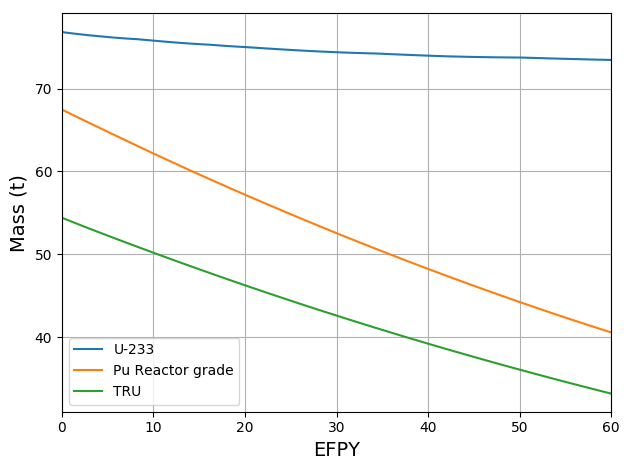
\includegraphics[width=\textwidth]{Th232CC.png}
	\caption{Mass variation of all thorium isotopes in the fuel salt for the $^{233}$U, reactor-grade Pu, and TRU cases.}
	\label{fig:Th232CC}
\end{figure}

Figure~\ref{fig:U233CC} demonstrates the mass of $^{233}$U in the fuel salt 
for the $^{233}$U, reactor-grade Pu, and TRU cases. The mass of 
$^{233}$U reaches equilibrium after $\approx$ $30$ years; overall, the 
amount of $^{233}$U is sufficient to maintain criticality in 
the three cases.
\begin{figure}
	\centering
	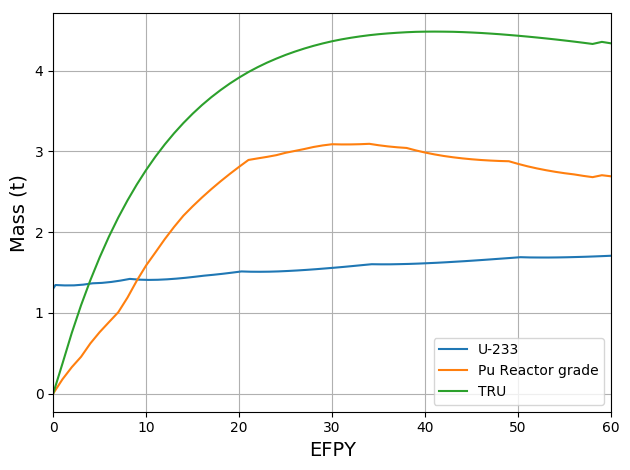
\includegraphics[width=\textwidth]{U233CC.png}
	\caption{Mass of $^{233}$U in the fuel salt for the $^{233}$U, reactor-grade Pu, and TRU cases.}
	\label{fig:U233CC}
\end{figure}

In the non-thorium feed mechanism, the SD-TMSR is continuously refueled by heavy metals (Pu and TRU) for 
criticality, which increases the Pu mole concentration (\%) in the molten salt. 
The Pu solubility in FLiBe is 
$\approx$ $4.0$ \% \cite{ignatiev2012progress,sood1975plutonium}. 
Figure~\ref{fig:PusolubilityCC} represents the Pu mole concentration variation in the fuel salt 
for the $^{233}$U, reactor-grade Pu, and TRU cases, respectively. In the $^{233}$U and reactor-grade Pu cases, the Pu mole concentration increases 
slightly but still below its solubility limit. On the other hand, the Pu 
mole concentration in the molten salt loaded by TRU increases during operation and 
reaches the Pu solubility limit after $\approx$ $40$ years. This issue may 
be solved by increasing the reactor operation temperature or reducing the 
HM initial inventory \cite{zou2018transition}.
\begin{figure}
	\centering
	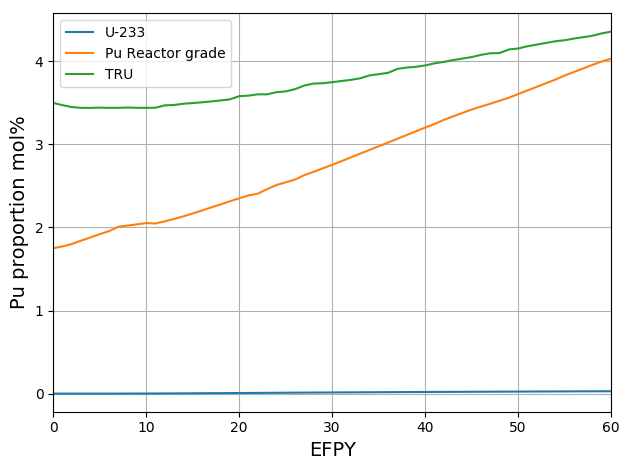
\includegraphics[width=\textwidth]{PusolubilityCC.png}
	\caption{The Pu mole concentration in the fuel salt for the $^{233}$U, reactor-grade Pu, and TRU cases.}
	\label{fig:PusolubilityCC}
\end{figure}
\FloatBarrier

Figure~\ref{fig:NetCC} demonstrates the net production of $^{233}$U during 
reactor operation for the $^{233}$U, reactor-grade Pu, and TRU cases, respectively. For the TRU case, the net production of $^{233}$U is almost 
zero. 
Although all produced $^{233}$U is used to refuel the core, the reactor is subcritical after $40$ years of operation (see Figure~\ref{fig:keff2}).
In the $^{233}$U and reactor-grade Pu cases, the net production of 
$^{233}$U increases with burnup and reaches about $1.77$ $t$ and $10$ $t$ at EOL, respectively. Figure~\ref{fig:NetCC} shows that for the $^{233}$U 
case the net production of $^{233}$U during the first 455 days is negative; 
about $175.28$ $kg$ of $^{233}$U must be added during this period. 
As shown in Figure~\ref{fig:NetCC}, for the $^{233}$U case, after 26 years the net production of $^{233}$U reaches 
$1.3$ $t$; this is sufficient to start up another \gls{SD-TMSR}. Similarly, 
one can see that the same amount of $^{233}$U ($1.3$ $t$) can be achieved 
after $\approx$ $4.5$ years if we apply the non-thorium feed mechanism on 
the SD-TMSR that was initially loaded by reactor-grade Pu alternative to 
$^{233}$U. For nonproliferation reasons, $^{233}$U could be diluted with $^{238}$U which makes it impossible to use for nuclear weapons.
  
In conclusion, the thorium fuel cycle transition can be achieved by selecting the 
proper feed mechanism and initial fissile material. 
Specifically, applying the non-thorium feed mechanism on 
the SD-TMSR loaded by reactor-grade Pu allows the 
transition to the thorium fuel cycle after $\approx$ 
$4.5$ years. Additionally, applying the thorium feed mechanism on 
the SD-TMSR loaded by $^{233}$U allows the 
transition to the thorium fuel cycle after $\approx$ $26$ years of operation. 
The comparison between the two feed mechanisms with various initial fuel types 
is listed in Table~\ref{tab:comp_feeds}. 

\begin{figure}
	\centering
	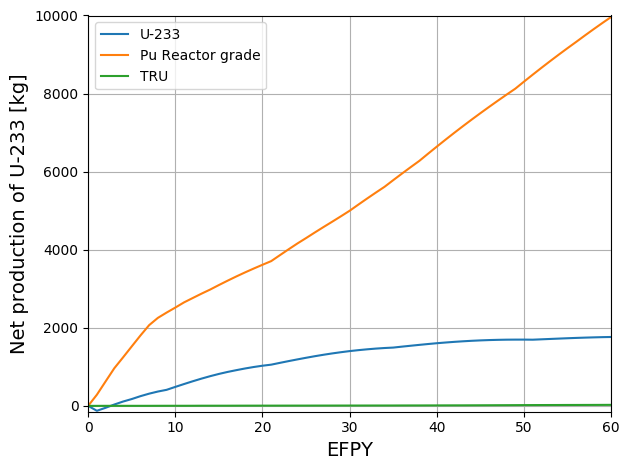
\includegraphics[width=\textwidth]{NetCC.png}
	\caption{Net production of $^{233}$U with burnup (60 \gls{EFPY}) for the $^{233}$U, reactor-grade Pu, and TRU cases.}
	\label{fig:NetCC}
\end{figure}

\begin{table}  [!h]
	\begin{minipage}{\linewidth}
		\renewcommand\footnoterule{}
		\renewcommand{\thefootnote}{\alph{footnote}}
		\caption{Comparison between the two feed mechanisms for the five different 
			types of initial fuel.}
		\label{tab:comp_feeds}
		\vspace{0.1in}
		\begin{tabularx}{\textwidth}{p{0.22\textwidth} X p{0.18\textwidth} 
				p{0.14\textwidth} X X 
			}  %{\textwidth}
			\hline
			Feed mechanism & \gls{HALEU} (19.79\%) & Pu+\gls{HALEU} (19.79wt.\%) &  
			reactor-grade Pu & \gls{TRU}& $^{233}$U \\
			\hline
			Thorium feed\\ mechanism&\xmark&\xmark&\xmark&\xmark& \cmark \\
			Non-thorium feed\\ mechanism &\xmark&\xmark&\cmark\footnotemark[1] 
			&\cmark\footnotemark[2] & \xmark\footnotemark[3] \\
			\hline
		\end{tabularx}
		\vspace{-1.5ex}%
		\footnotetext[1]{Positive $^{233}$U net production and critical 
			configuration for 60 years of operation.}
		\footnotetext[2]{Zero $^{233}$U net production and critical 
			configuration for 40 years of operation.}		
		\footnotetext[3]{Too large and increasing $k_{eff}$ during 
			lifetime.}		
	\end{minipage}
\end{table}
\FloatBarrier

\subsection{Neutron spectrum}
Figure~\ref{fig:spectrumFLUX110vC} represents the neutron flux per unit 
lethargy for a full-core SD-TMSR model in the energy range from 10$^{-8}$ to 
10 MeV for the $^{233}$U, reactor-grade Pu, and TRU cases at BOL and EOL. In 
the $^{233}$U case, at the EOL, the neutron spectrum is harder than at BOL due 
to the accumulation of Pu and other strong thermal neutron absorbers in the 
fuel salt. For the reactor-grade Pu and TRU cases, during reactor operation, 
the fissile Pu is depleted and the $^{233}$U becomes the major fissile isotope 
(see Figure~\ref{fig:U233CC}); the neutron spectrum softens and becomes 
similar to the initial thermal spectrum of a $^{233}$U fueled \gls{SD-TMSR}.
 \begin{figure}
 	\centering
 	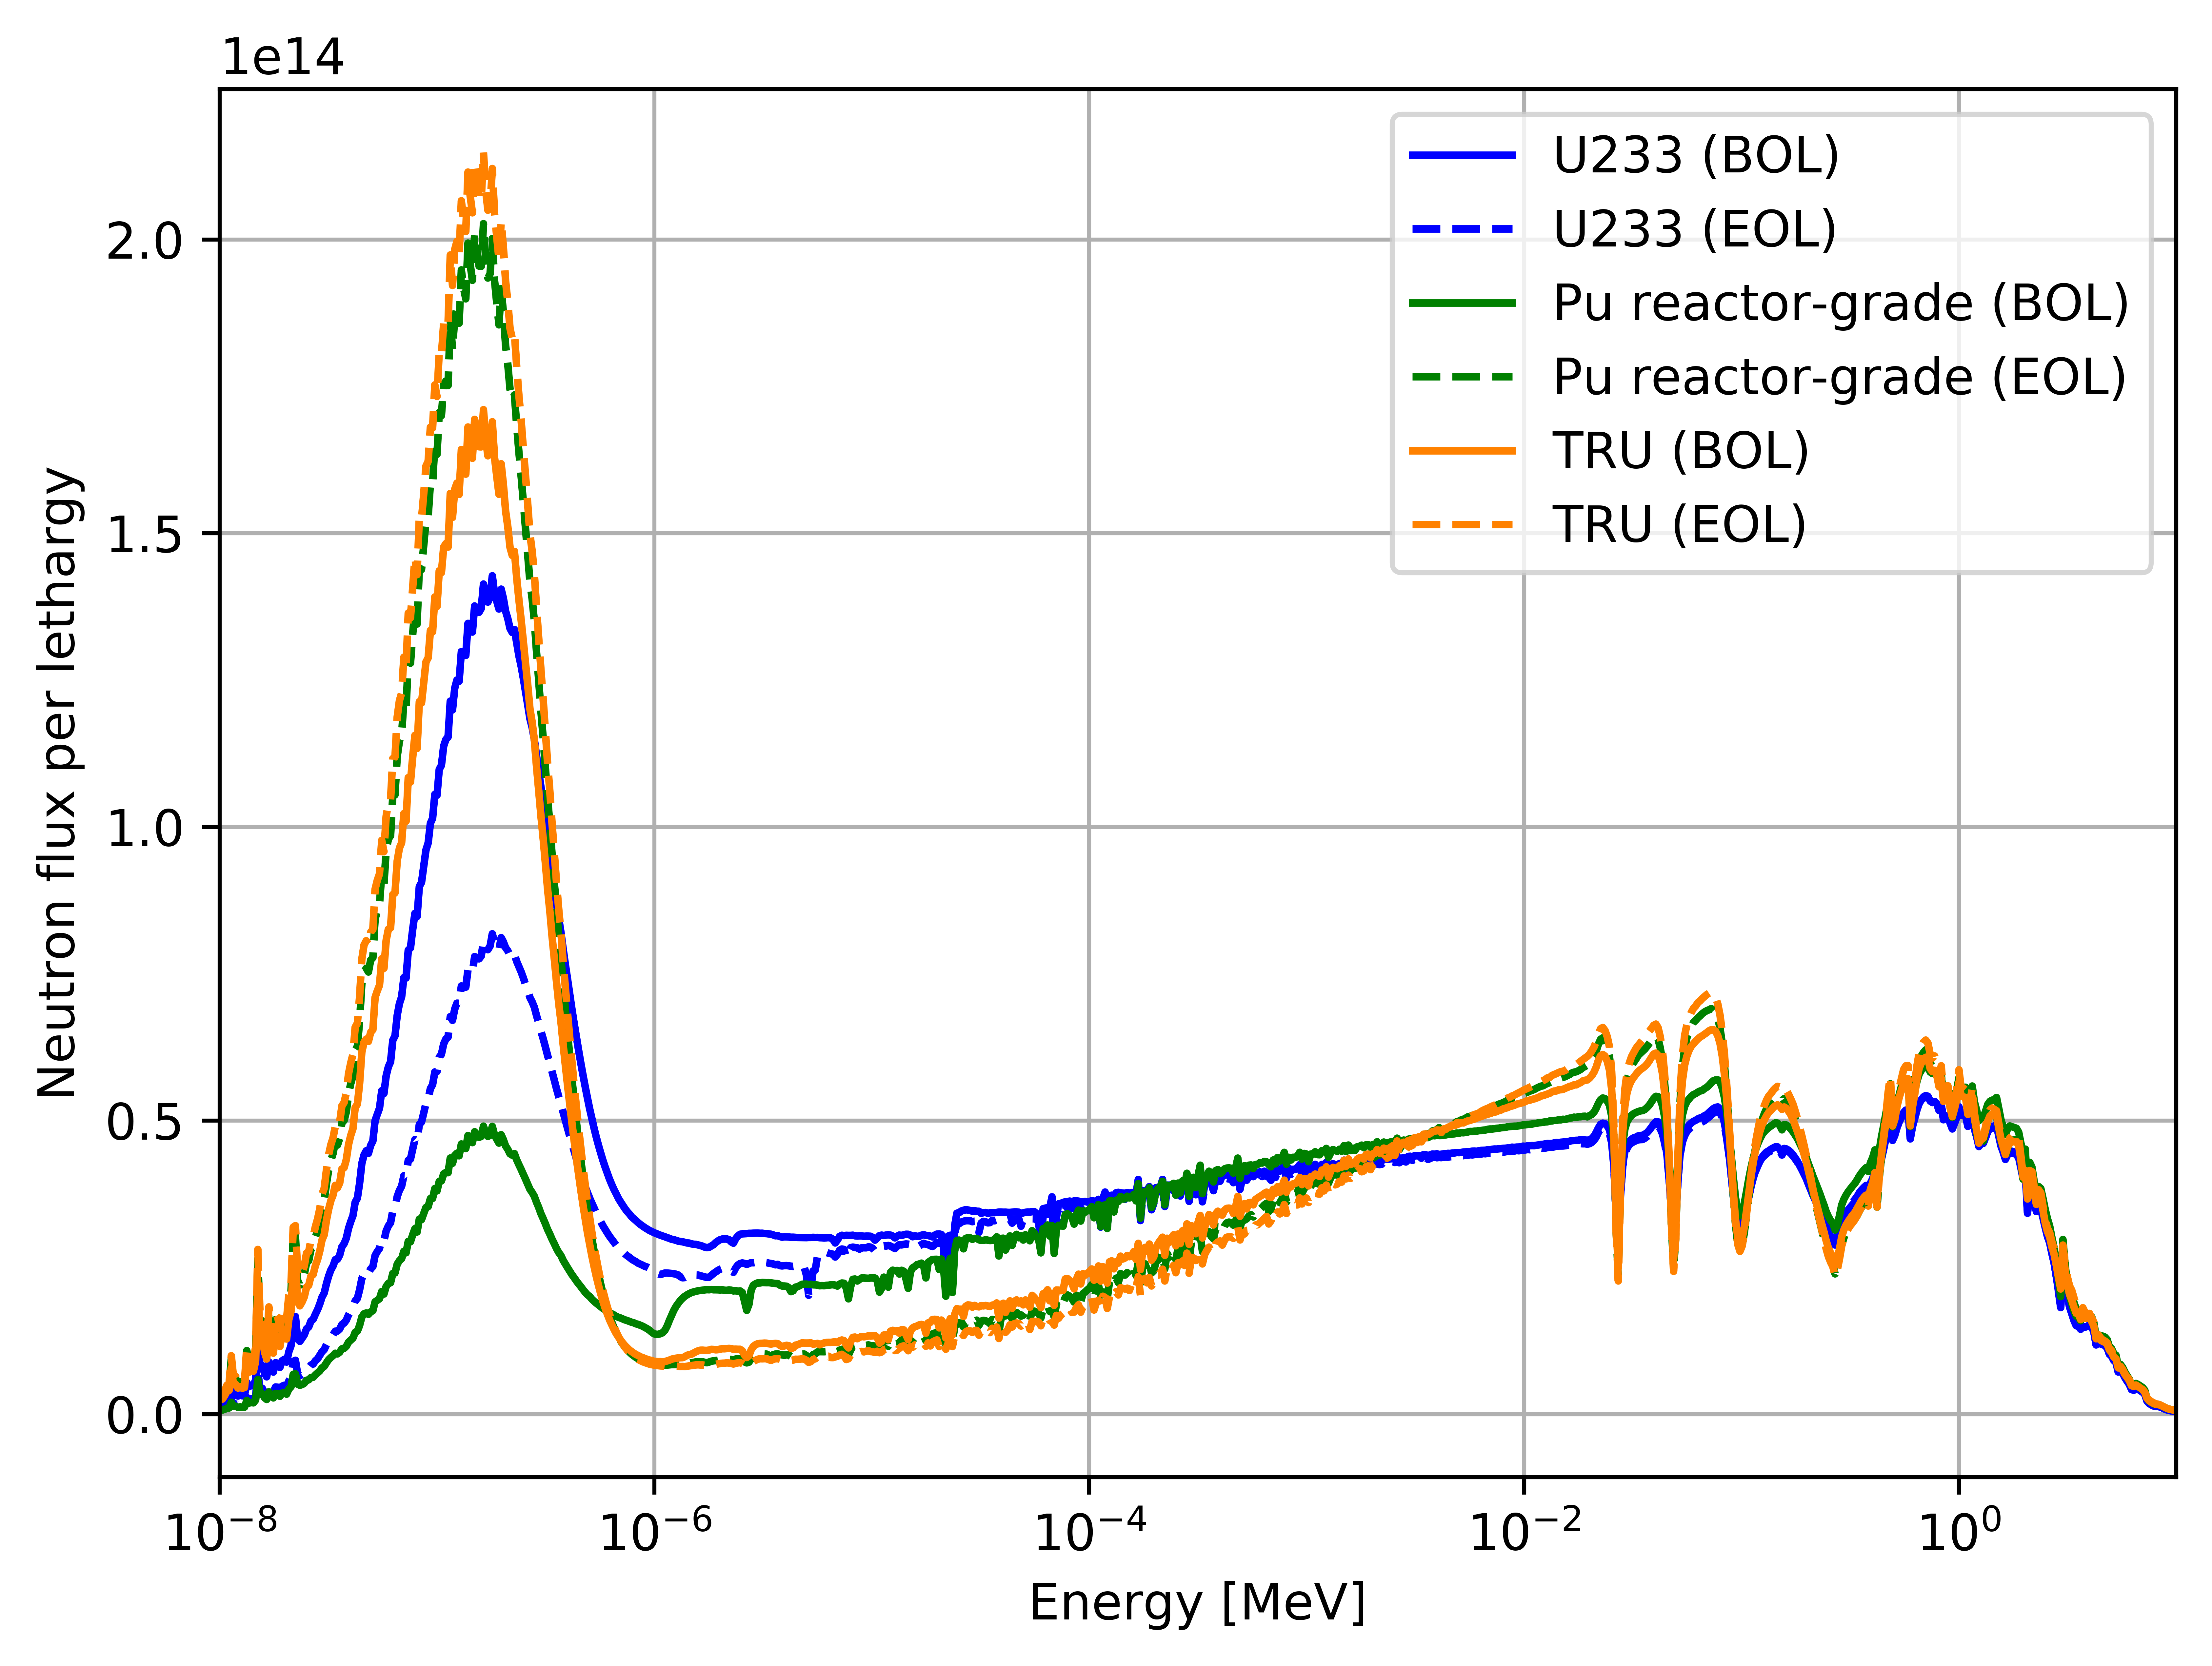
\includegraphics[width=1.01\textwidth]{spectrumFLUX110vC.png}
 			\vspace{-0.4in}
 	\caption{The neutron flux energy spectrum at BOL (solid lines) and EOL (dashed lines) for 3 different initial 
 		fuel salt compositions (for all cases, the neutron flux
 		confidence intervals $\pm\sigma$ at BOL and EOL are $<1.0139$\% and $<0.6274$\%, respectively).}
 	\label{fig:spectrumFLUX110vC}
\end{figure}

\subsection{Neutron flux}
Figures~\ref{fig:fast_flux} and \ref{fig:thermal_flux} show the radial 
distribution of fast (energy range between 0.625 eV and 20 MeV) and thermal 
(energy range between 10$^{-5}$ eV and 0.625 eV) neutron flux for three 
different initial fissile materials in the fuel salt ($^{233}$U, reactor-grade 
Pu, TRU) at startup and at equilibrium (after $\approx 30$ years of 
operation). Actinides' evolution and poisonous fission product accumulation 
for various initial fissile compositions demonstrates the different effects on 
the SD-TMSR neutronics performance. For the $^{233}$U case, the thermal 
neutron flux is suppressed at equilibrium because fissile $^{233}$U in the 
core is being substituted with heavier fissile actinides: $^{235}$U, 
$^{239}$Pu, and $^{241}$Pu. This agrees with results in literature 
\cite{rykhlevskii2019modeling, ashraf2019whole_core}.
\begin{figure}[htp!] % replace 't' with 'b' to force it to \centering
	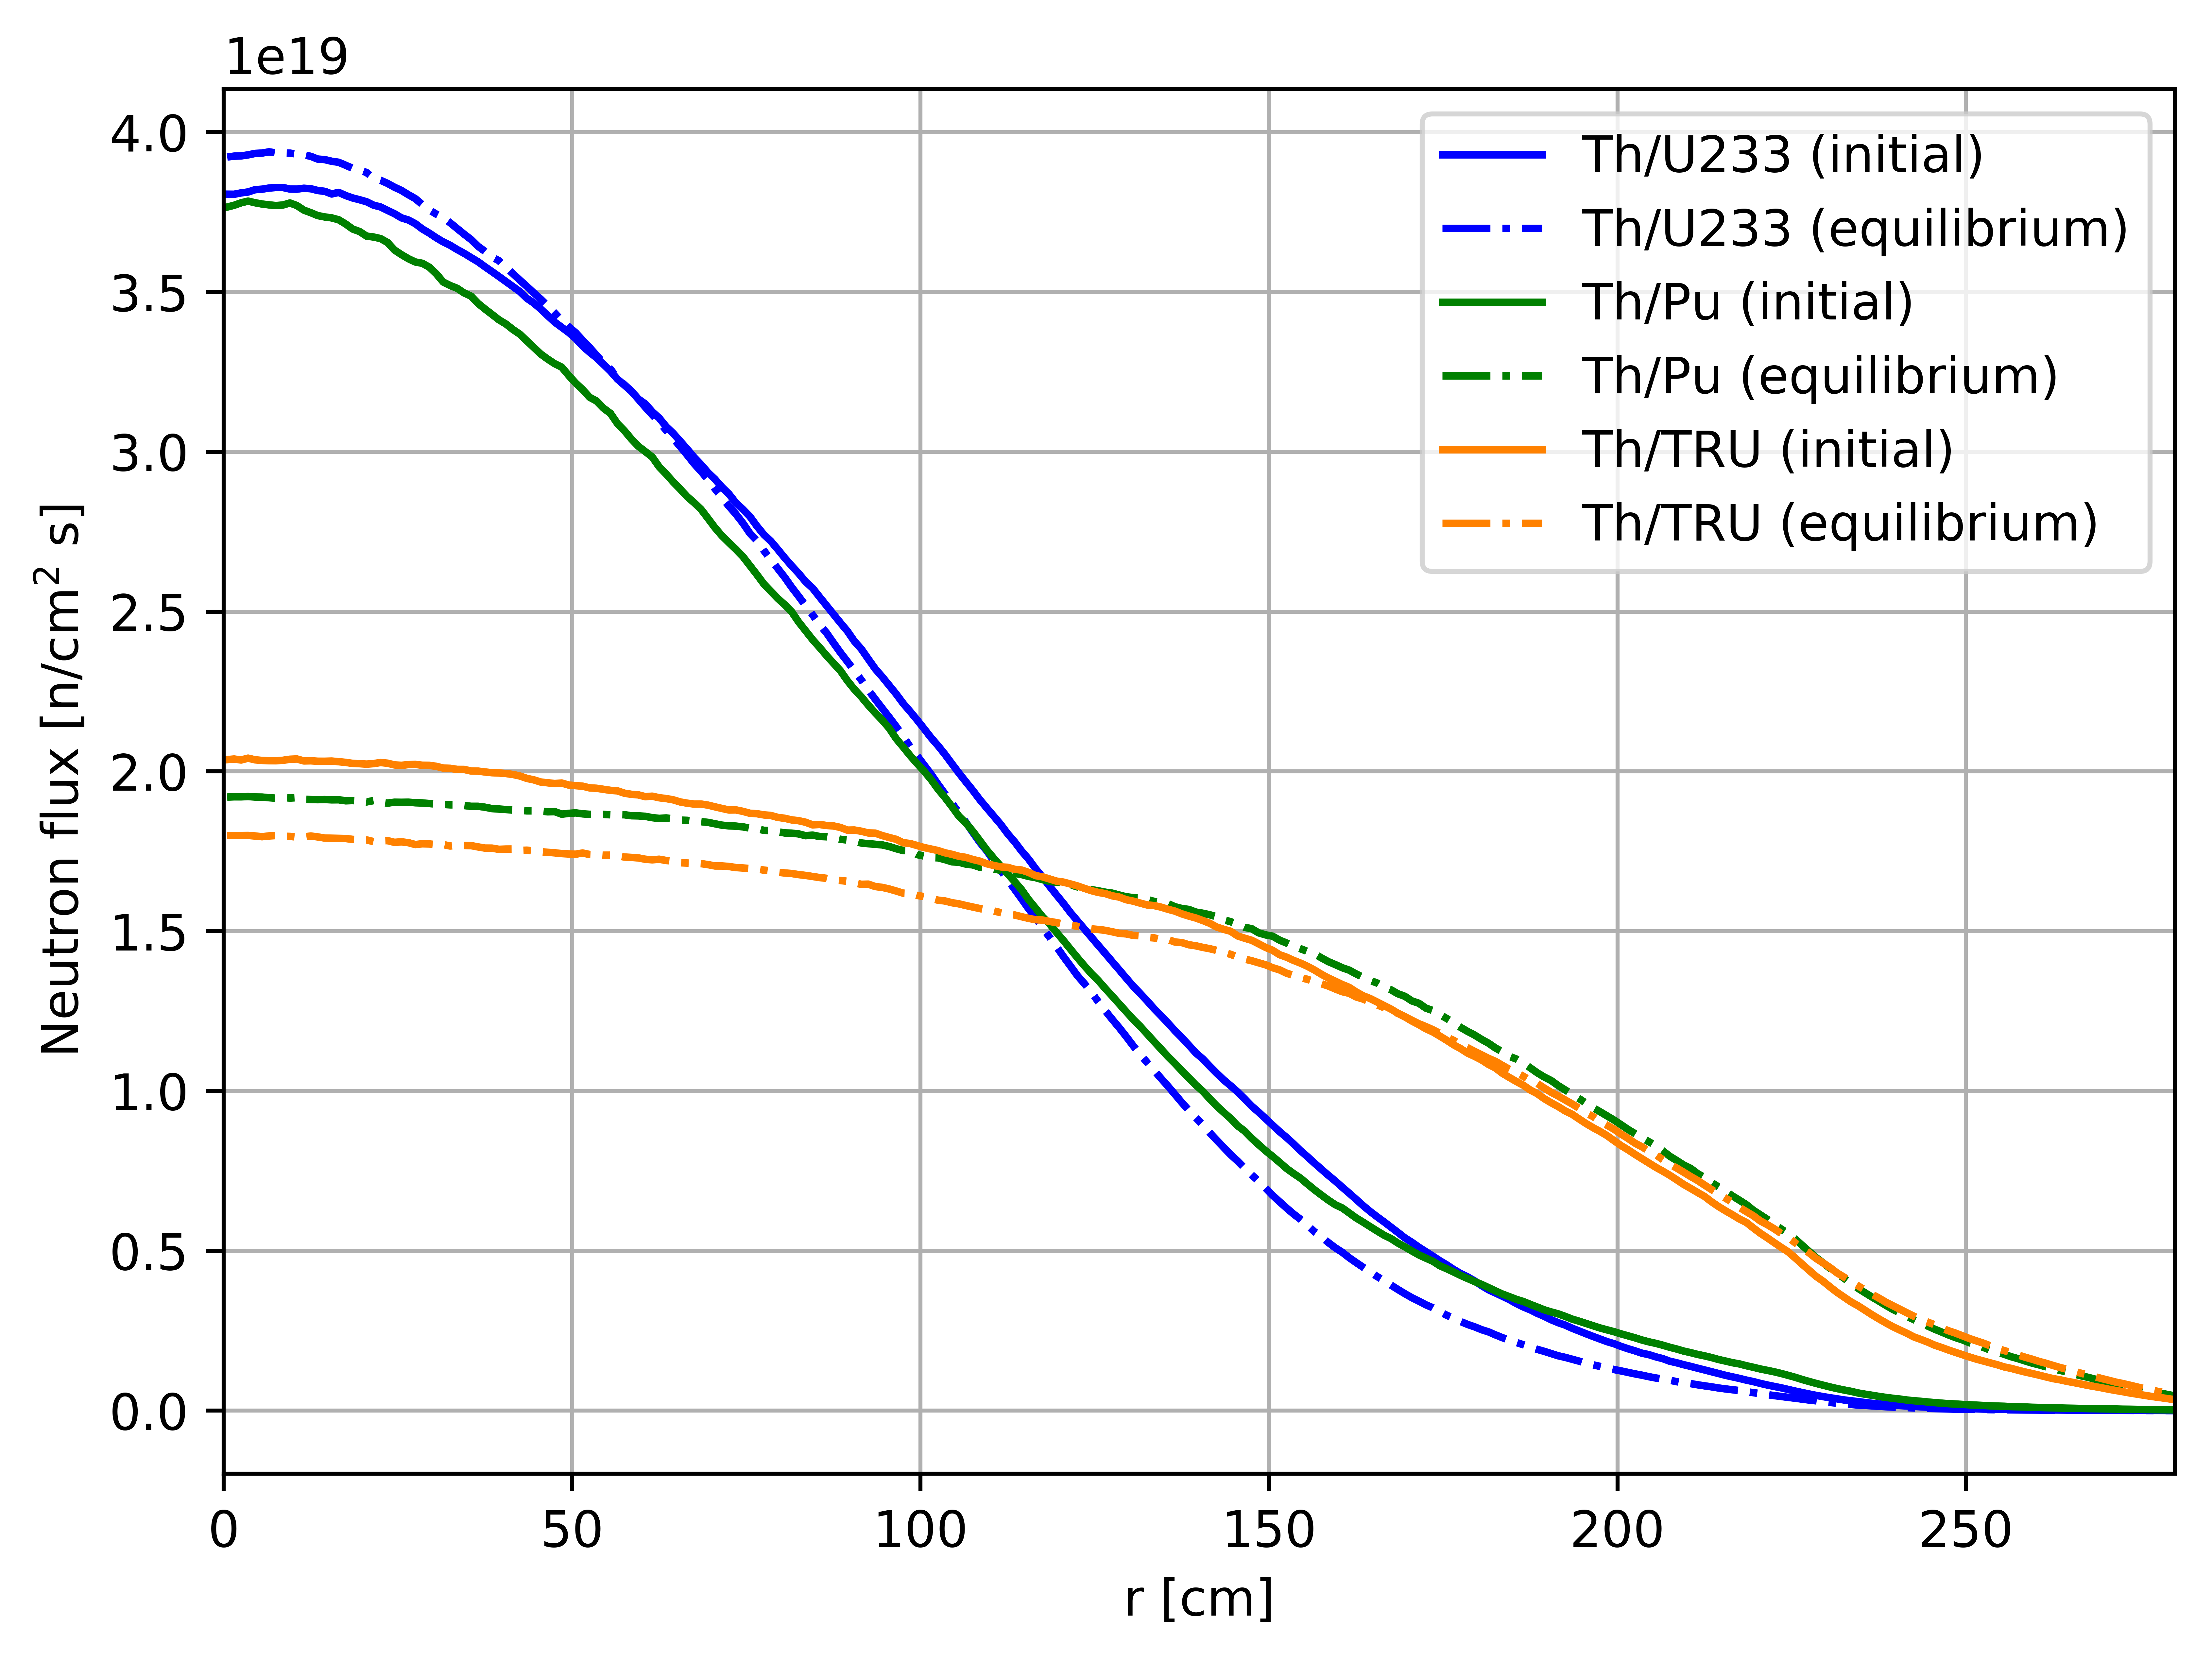
\includegraphics[width=\textwidth]{radial_fast_flux_init_vs_eq.png} 
	\caption{Radial fast neutron flux distribution for 3 different initial 
		fuel salt compositions at startup and equilibrium (the fast flux 
		confidence interval $\pm\sigma<2.5$\% for all cases).}
	\label{fig:fast_flux}
\end{figure}

Opposite behavior is observed for the reactor-grade Pu and TRU cases. For  
these cases, the thermal neutron flux increases during operation while fast 
neutron flux decreases. Fissile Pu nuclides (generate relatively hard 
spectrum) from initial fuel salt composition are gradually substituted with  
$^{233}$U (generates relatively soft spectrum), produced from fertile 
$^{232}$Th. During reactor operation, $^{233}$U becomes the primary fissile 
isotope, which softening the neutron spectrum of the reactor. 
\begin{figure}[htp!] % replace 't' with 'b' to force it to \centering
	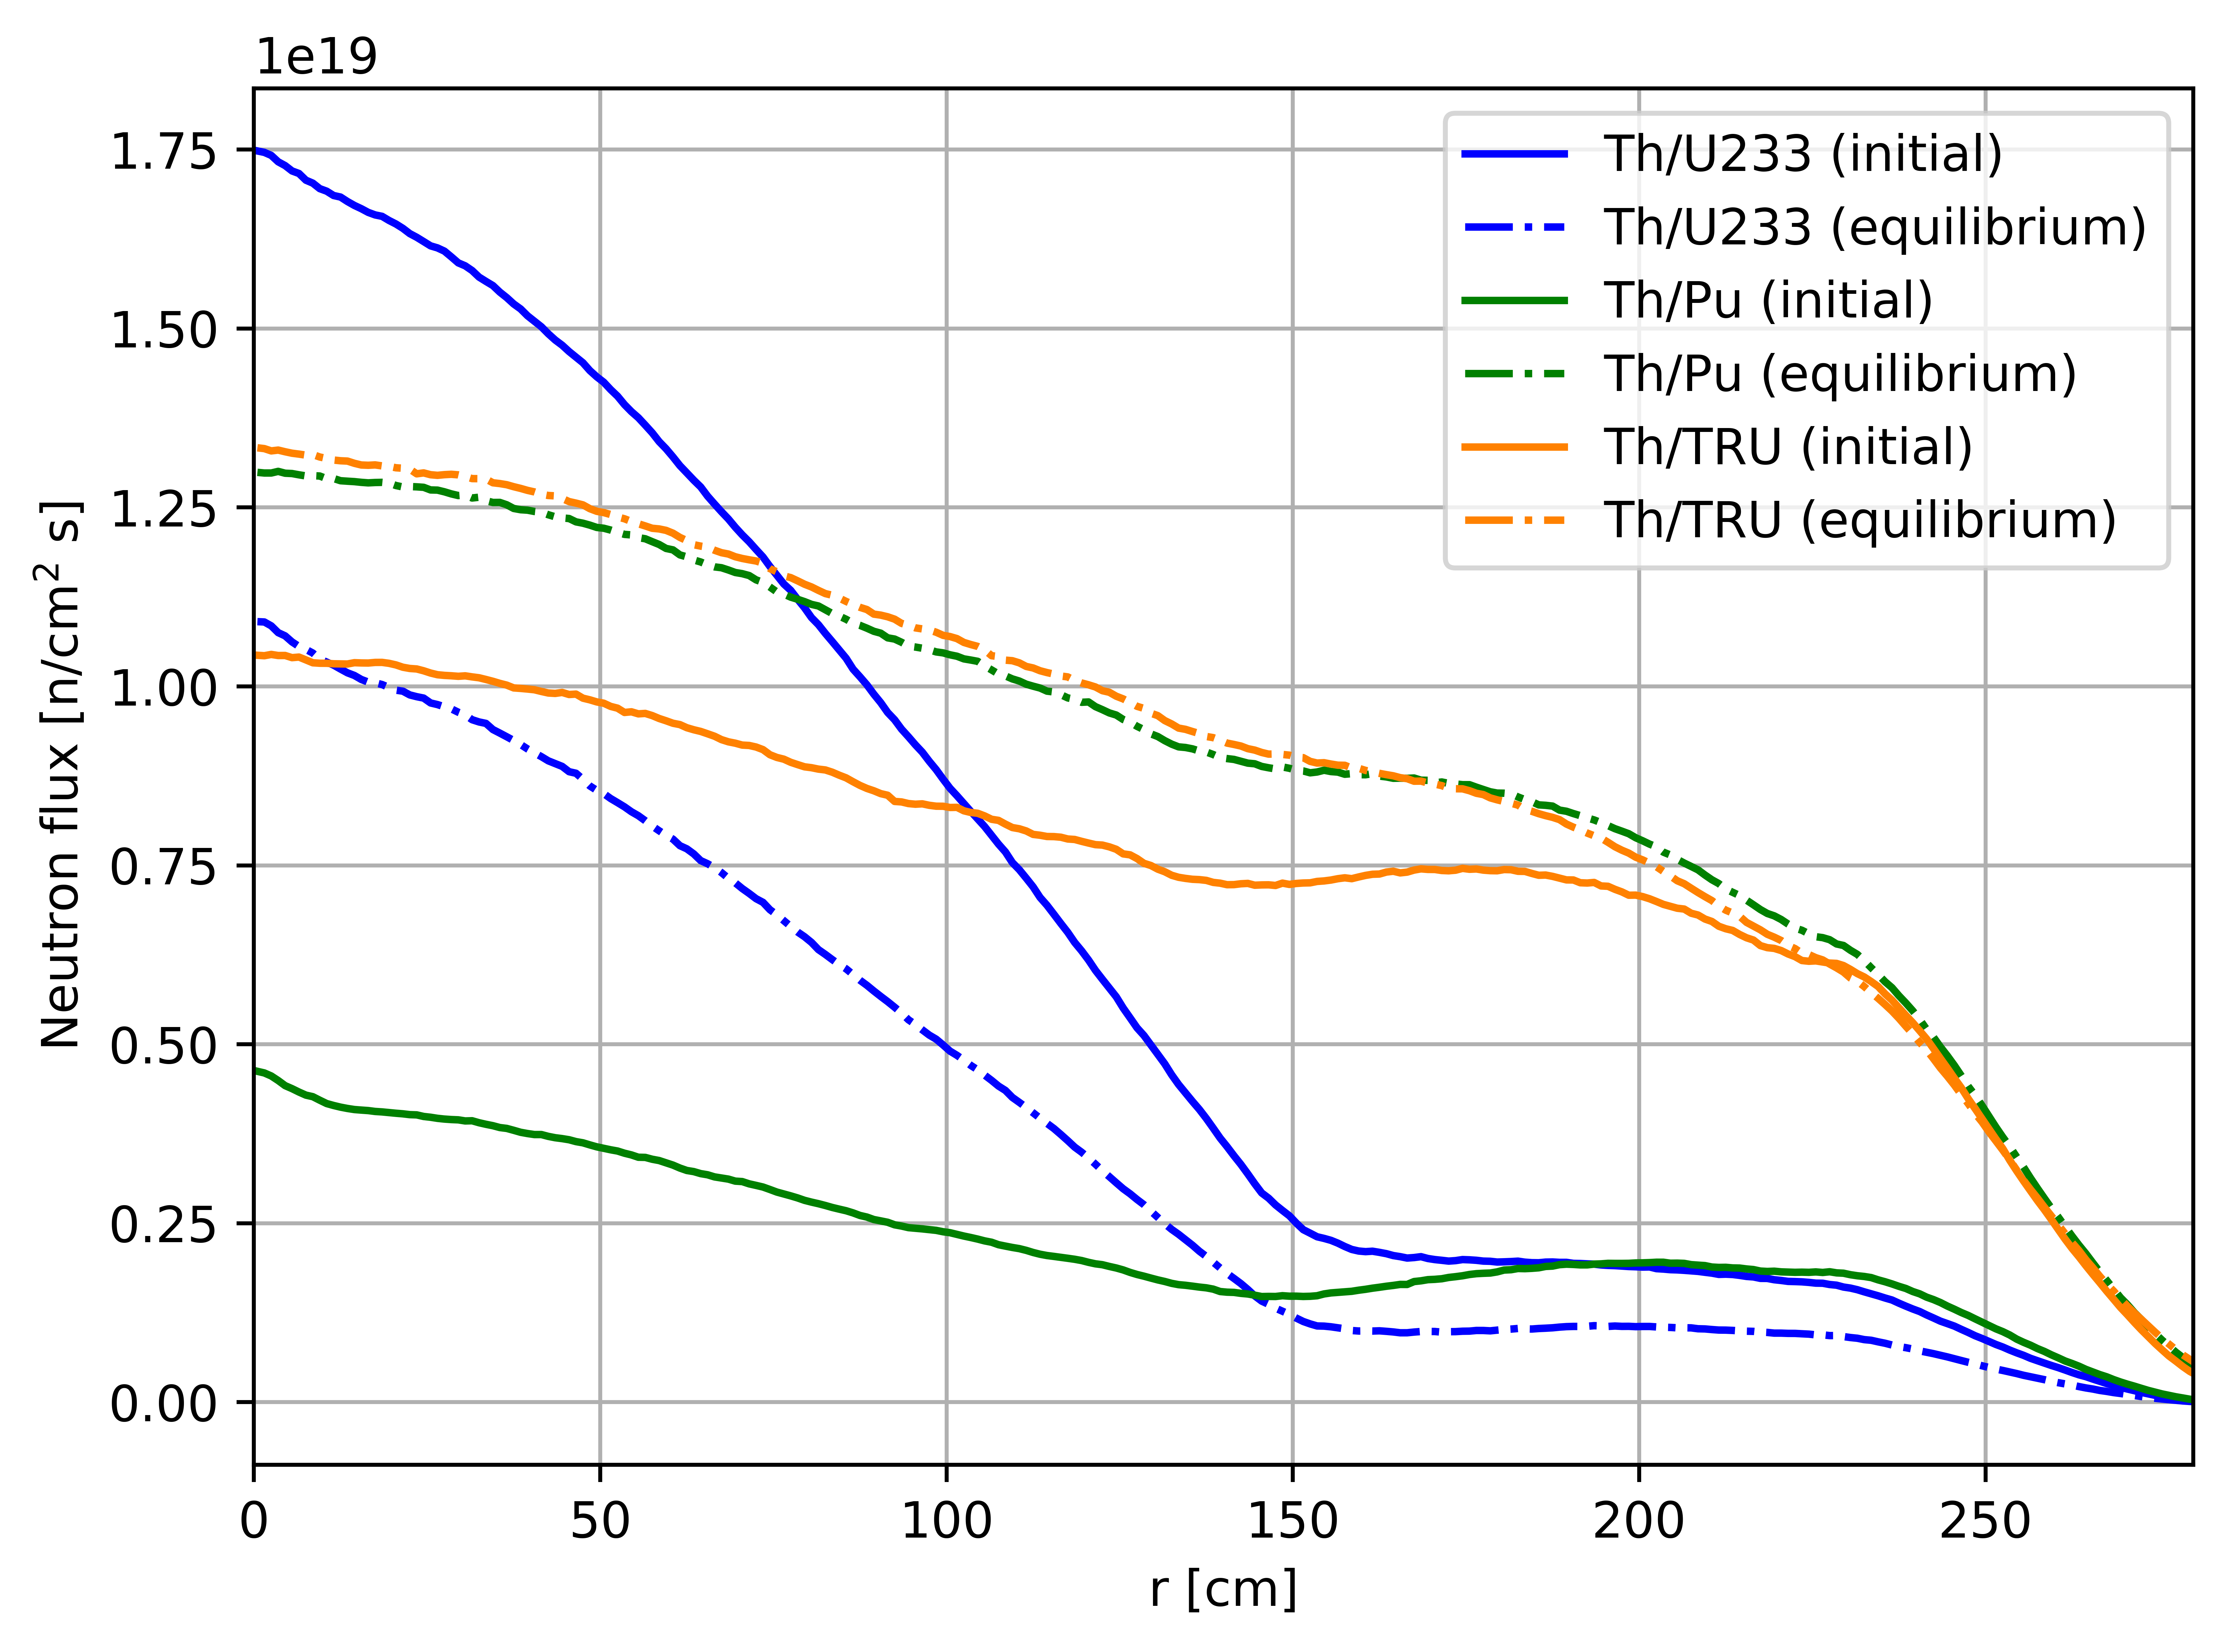
\includegraphics[width=\textwidth]{radial_thermal_flux_init_vs_eq.png} 
	\caption{Radial thermal neutron flux distribution for 3 different initial 
		fuel salt compositions at startup and equilibrium (the thermal flux 
		confidence interval $\pm\sigma<1.6$\% for all cases).}
	\label{fig:thermal_flux}
\end{figure}

More changes in thermal neutron flux shape and magnitude for the 
$^{233}$U case are observed in the inner core zone ($R\lesssim150$) than 
in the outer core zone. In contrast, for the reactor-grade Pu and TRU cases, 
significant changes are observed for thermal neutron flux in the outer core 
zone and reflector. Additionally, Figure~\ref{fig:thermal_flux} shows 
relatively large changes in thermal flux leakage from the core for the Pu and 
TRU cases. The SD-TMSR core design was optimized for $^{233}$U  
\cite{li_optimization_2018}, thus, the core geometry (e.g., channels lattice 
pitch) must be re-optimized for another type of fuel to obtain better 
neutronics performance.

\subsection{Temperature coefficient of reactivity}
The temperature coefficient of reactivity quantifies reactivity changes due to 
temperature increase in the core and is calculated in this work as follows:
\begin{align}
\alpha &= \frac{k_{eff}(T_{i+1}) - k_{eff}(T_i)}{k_{eff}(T_{i+1}) 
	k_{eff}(T_{i}) (T_{i+1} - T_i)}
\intertext{where}
k_{eff} &= \mbox{effective multiplication factor} \nonumber \\
T_i &= \mbox{fuel salt temperature in (900 K, 1000 K).} \nonumber
\end{align}

Table~\ref{tab:tcoe} summarizes temperature coefficients calculated for three 
different initial fissile loads at startup and at equilibrium. By propagating 
the $k_{eff}$ statistical error provided by SERPENT-2, uncertainty for each 
temperature coefficient is calculated using the following formula:
\begin{align}
\delta\alpha &= \abs{\frac{1}{T_{i+1} - T_i}} \sqrt{\frac{\delta 
		k_{eff}^2(T_{i+1})}{k_{eff}^4(T_{i+1})}  
	+ \frac{\delta k_{eff}^2(T_i)}{k_{eff}^4(T_i)}}
\intertext{where}
\delta k_{eff} &= \mbox{statistical error for $k_{eff}$ from SERPENT-2 
output.} 
\nonumber
\end{align}

Other sources of uncertainty are neglected, such as cross section measurement 
error and approximations inherent in the density dependence on temperature. 

When the fuel salt temperature increases, the density of the salt decreases, 
but at the same time, the total volume of fuel salt in the 
core remains constant because it
is bounded by the vessel. When the graphite 
temperature increases, the density of
graphite decreases, creating additional 
space for the salt. The cross section temperatures for the fuel and moderator 
were changed from 900 to 1000 K to determine the temperature coefficients. 
This work considered five different cases:
\begin{enumerate}
	\item Fuel salt temperature (Doppler Effect) rising from 900 to 1000 K 	
	(first row in Table~\ref{tab:tcoe}).
	\item Fuel salt density decreasing from 3.3 to 3.233 g/cm$^3$ 
	(density change caused by temperature increase from	900 to 1000 K).
	\item Total fuel salt temperature (Doppler+density) rising from 900 to 
	1000 K.	
	\item Graphite temperature (Doppler Effect) rising from 900 to 1000 K.
	\item Whole reactor temperature rising from 900 K to 1000 K.
\end{enumerate}

In the first case, the fuel temperature change only impacts cross section 
temperature. In the second case, changes in the fuel temperature only impact 
density, and the third case takes into account both effects. The geometry for 
these three cases is unchanged because the fuel is a liquid. However, when 
the graphite blocks heat up, both the density and the geometry change due 
to the thermal expansion of solid graphite. The graphite linear thermal 
expansion is not a dominating factor \cite{li_optimization_2018}, and herein 
we focus only on the Doppler Effect for the moderator temperature coefficient.
%%%%%%%%%%%%%%%%%%%%%%%%%%%%%%%%%%%%%%%%
\begin{table} [b!]
	\caption{Temperature coefficients of reactivity for 3 different initial 
		fuel salt compositions at startup and equilibrium. Confidence interval 
		$\pm\sigma$ for all coefficients is between $0.11$ and $0.16$ pcm/K).}
	\begin{tabularx}{\textwidth}{ p{0.27\textwidth} | X X  X X  X X } \hline
		\multirow{3}{*}{\shortstack{Reactivity coefficient \\ (pcm/K)}} 
		& 
		\multicolumn{6}{c}{Startup fissile material} \\ \cline{2-7}
		\space  & \multicolumn{2}{c}{$^{233}U$} & \multicolumn{2}{c}{Pu} & 
		\multicolumn{2}{c}{TRU} \\ \cline{2-7}
		\space  & Initial & Equil. & Initial & Equil. & Initial & 
		Equil. \\ \hline
		Fuel salt temperature ($\alpha_{D,fuel}$) &$-4.96$&$-5.26$&$-4.99$&$-3.12$&$-3.23$&$-1.97$ 
		\\ 
		Fuel salt density ($\alpha_{l,fuel}$) &$+1.49$&$+2.34$&$+1.54$&$-1.58$&$-0.37$&$-1.62$ \\
		Total salt fuel ($\alpha_{fuel})$ &$-3.77$&$-2.83$&$-3.22$&$-4.23$&$-3.25$&$-3.69$ \\ 
		\hline
		Graphite temperature ($\alpha_{D,M}$) &$+1.45$&$+0.45$&$-2.68$&$-1.37$&$-1.44$&$-1.14$ 
		\\	\hline
		Total core ($\alpha$) &$-1.77$&$-2.59$&$-6.54$&$-5.06$&$-4.79$&$-4.76$ \\ \hline
	\end{tabularx}
	\label{tab:tcoe}
\end{table}
%%%%%%%%%%%%%%%%%%%%%%%%%%%%%%%%%%%%%%%%%%%%%%%%%%%%%%%%%%%%%%%%%%%%%%%%%%%%%%%%

The \gls{FTC} is negative for all considered fuel compositions due to thermal 
Doppler broadening of the resonance capture cross sections in the thorium. For 
the $^{233}$U case, the \gls{FTC} decreases in magnitude by $25\%$ due to 
neutron spectrum hardening during the reactor operation. For reactor-grade Pu 
and TRU cases, the \gls{FTC} increases in magnitude at equilibrium, by $31\%$ 
and $14\%$, respectively. Spectrum softening for these fueling cases 
positively affects the \gls{FTC} magnitude, and this effect seems to be 
proportional to the spectrum shift.

The \gls{MTC} for the $^{233}$U case is positive and decreases during reactor 
operation because of spectrum hardening with fuel depletion. For other cases, 
the \gls{MTC} is negative and also decreases in magnitude during reactor  
operation. Finally, the total temperature coefficient of reactivity is 
strongly negative for all considered scenarios but decreases in magnitude 
during reactor operation due to spectral shift. Notably, the total temperature 
coefficient is the most negative for the reactor-grade Pu case at startup, 
which has the hardest neutron spectrum (Figure~\ref{fig:spectrumFLUX110vC}). 
These coefficients agree with earlier estimates for the SD-TMSR 
\cite{li_optimization_2018, ashraf2019whole_core} and \gls{MSBR} 
\cite{rykhlevskii2019modeling, rykhlevskii_full-core_2017,  
robertson_conceptual_1971}.

Even after 30 years of operation, the total temperature coefficient of 
reactivity remains relatively large and negative (in the range between $-2.59$ 
and $-5.06$ pcm/K) compared to the conventional \gls{PWR}, which has 
temperature coefficient of about $-1.71$ $pcm/^{\circ}F\approx -3.08$ $pcm/K$ 
\cite{forget_integral_2018}, and allows excellent reactor stability and 
control. The additional analysis must be performed taking graphite moderator 
density change and linear thermal expansion into account, but material 
properties for the SD-TMSR graphite are not available in published literature. 
Relatively well-studied reactor graphite (e.g., AXQ graphite 
\cite{robertson_conceptual_1971}) can be considered as a candidate for the 
SD-TMSR concept.

\subsection{Six factor analysis}
The effective multiplication factor can be expressed as follows:
\begin{align}
k_{eff} &= \eta f p \epsilon P_f P_t
\intertext{where}
\eta     &= \mbox{neutron reproduction factor} \nonumber \\
f        &= \mbox{thermal utilization factor} \nonumber \\
p        &= \mbox{resonance escape probability} \nonumber \\
\epsilon &= \mbox{fast fission factor} \nonumber \\
P_f      &= \mbox{fast non-leakage probability} \nonumber \\
P_t      &= \mbox{thermal non-leakage probability.} \nonumber
\end{align}

Table~\ref{tab:six_factor} summarizes the six factor for 3 different initial 
fuel salt compositions at startup and equilibrium. By using SERPENT-2 built-in 
online reprocessing capabilities, six factor is calculated at the 
beginning of the operation and after 30 years of operation. Neutron population 
and number of active/inactive cycles were selected to obtain $k_{eff}$ 
statistical uncertainty less than 12 pcm. The fast and thermal non-leakage 
probabilities remain constant regardless of initial fissile material and 
neutron spectrum shift during operation. The thermal utilization factor (f) 
remains almost constant during operation for the $^{233}$U and TRU cases but 
considerably declines for the Pu case due to significant neutron spectrum 
softening.
%%%%%%%%%%%%%%%%%%%%%%%%%%%%%%%%%%%%%%%%
\begin{table} [ht!]
	\caption{Six factor for the SD-TMSR model for 3 different initial 
		fuel salt compositions at startup and equilibrium.}
	\begin{tabularx}{\textwidth}{ X | X X  X X  X X } \hline
		\multirow{3}{*}{Factor}  & \multicolumn{6}{c}{Startup fissile 
			material} \\ \cline{2-7}
		\space  & \multicolumn{2}{c}{$^{233}U$} & \multicolumn{2}{c}{Pu} & 
		\multicolumn{2}{c}{TRU} \\ \cline{2-7}
		\space  & Initial & Equil & Initial & Equil & Initial & Equil \\ \hline
		$\eta$  & 1.26 & 1.40 & 1.66 & 1.44 & 1.59 & 1.31 \\ 
		f       & 0.97 & 0.98 & 0.96 & 0.76 & 0.80 & 0.75 \\
		p       & 0.54 & 0.43 & 0.26 & 0.16 & 0.17 & 0.15 \\
		$\epsilon$ & 1.49 & 1.67 & 2.45 & 5.87 & 4.83 & 6.81 \\
		P$_f$   & 0.99 & 0.99 & 0.99 & 0.99& 0.99 & 0.99 \\
		P$_t$   & 1.00 & 1.00 & 1.00 & 1.00 & 1.00 & 1.00 \\ \hline
	\end{tabularx}
	\label{tab:six_factor}
\end{table}
%%%%%%%%%%%%%%%%%%%%%%%%%%%%%%%%%%%%%%%%%%%%%%%%%%%%%%%%%%%%%%%%%%%%%%%%%%%%%%%%

In contrast, the neutron reproduction factor ($\eta$), resonance escape 
probability ($p$), and fast fission factor ($\epsilon$) differ notably between 
the initial and equilibrium state for all three initial fissile materials.  
$\epsilon$ is much larger at startup for the Pu and TRU cases because these 
initial fissile materials provide a much harder neutron spectrum than 
$^{233}$U, and $\epsilon$ grows throughout the core's lifetime. Conversely, 
$p$ decreases during reactor operation. The neutron reproduction factor ($\eta$)  
increases during reactor operation for the $^{233}$U as initial fuel due to 
the accumulation of fissile plutonium isotopes, which produce more neutrons 
per fission ($\nu$). The other two scenarios demonstrate opposite behavior: 
plutonium isotopes with large $\nu$ are gradually substituted with $^{233}$U, 
which has a lower $\nu$ \cite{sjostrand_cross_1960}. This six factors' 
evolution agrees with previously determined evolution parameters for a similar 
single-fluid double-zone \gls{MSBR} \cite{ashraf2019whole_core, 
rykhlevskii2019modeling, park_whole_2015}.